\documentclass{article}
\usepackage{geometry}
 \geometry{
 a4paper,
 total={210mm,297mm},
 left=20mm,
 right=20mm,
 top=20mm,
 bottom=20mm,
 }

\usepackage[dvipsnames]{xcolor}
\usepackage{siunitx} % Provides the \SI{}{} command for typesetting SI units
\usepackage{listings}
\usepackage{graphicx} % Required for the inclusion of images
\usepackage{enumerate}
\usepackage{float}
\usepackage{fancyvrb}
\usepackage[utf8]{inputenc}
\usepackage{listings}
\usepackage{inconsolata}
\usepackage{placeins}
\usepackage{subcaption}
\usepackage[draft]{fixme}
\usepackage{float}
\usepackage{fontawesome}

\usepackage{hyperref}
\hypersetup{
  colorlinks   = true,    % Colours links instead of ugly boxes
  urlcolor     = blue,    % Colour for external hyperlinks
  linkcolor    = blue,    % Colour of internal links
  citecolor    = red      % Colour of citations
}

\newcommand{\codelink}[1]{%
    \hyperref[#1]{\quad\faArrowCircleRight\enskip Matlab Code (Listing~\ref{#1})}%
}

\lstset{
    basicstyle=\small\ttfamily,
    keywordstyle=\color{blue}\textbf\ttfamily,
    commentstyle=\color{OliveGreen}\textbf\ttfamily,
    frame=single,
    rulecolor=\color{black},    %%% <--- here
    breaklines=true,
}

\setlength\parindent{0pt} % Removes all indentation from paragraphs

\title{Network Security \\ 389.159 - SS 2018 \\ Lab Exercise 3 \& Lab Exercise 4} % Title

\author{
    TEAM 02 \\
    Corentin \textsc{Bergès} (11741629) (066 506) \\
    Christoph \textsc{Echtinger-Sieghart} (00304130) (066 938)
}

\date{\today} % Date for the report
\begin{document}

\maketitle % Insert the title, author and date
\renewcommand{\arraystretch}{2} %Stretch rows

%\listoffixmes

\section{Lab Exercise 3}

\subsection{rep-10 \codelink{code:rep-10}}

Figure~\ref{figure:rep-10} shows the stem plots for packets, bytes, unique IP sources and
unique IP destinations per hour.

\begin{figure}[H]
    \begin{subfigure}{.5\textwidth}
        \centering
        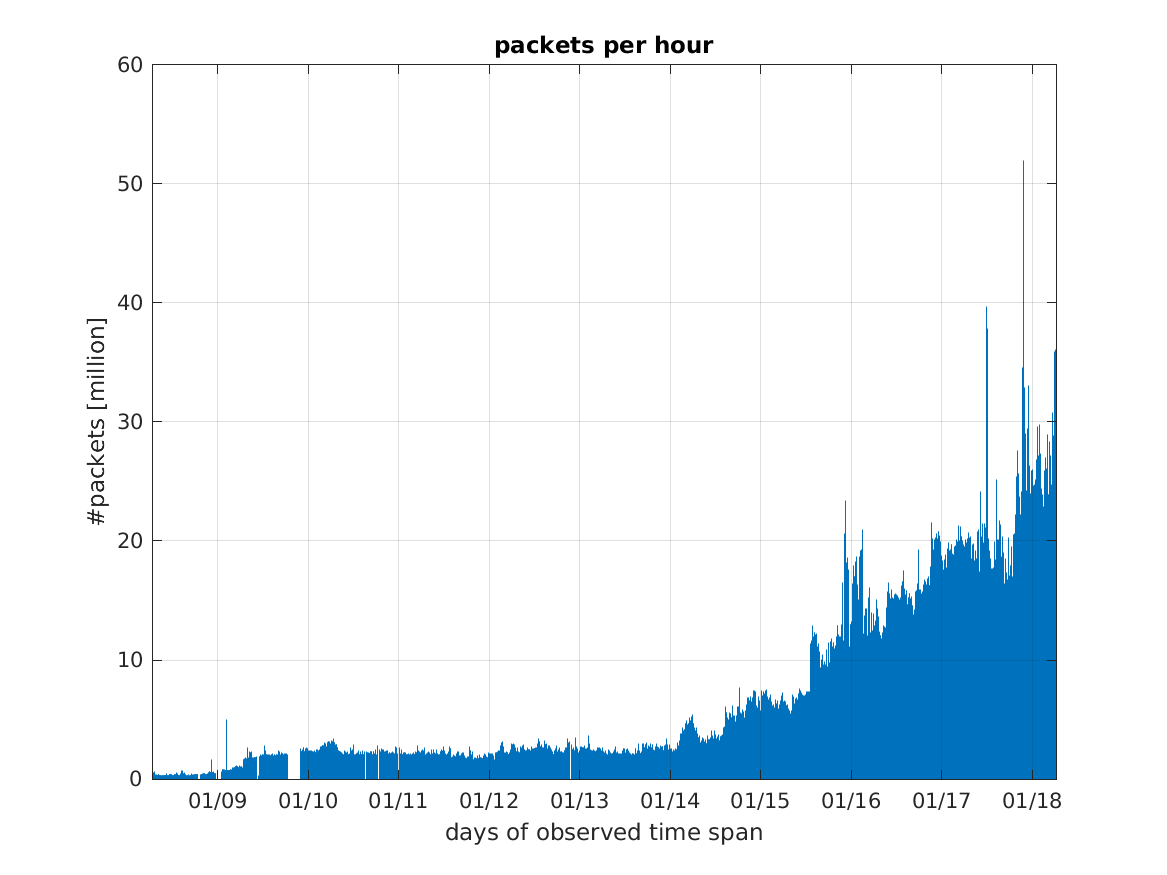
\includegraphics[width=\textwidth]{../exercise-3/plots/rep_10_1}
        \caption{Packets per hour}
    \end{subfigure}
    \begin{subfigure}{.5\textwidth}
        \centering
        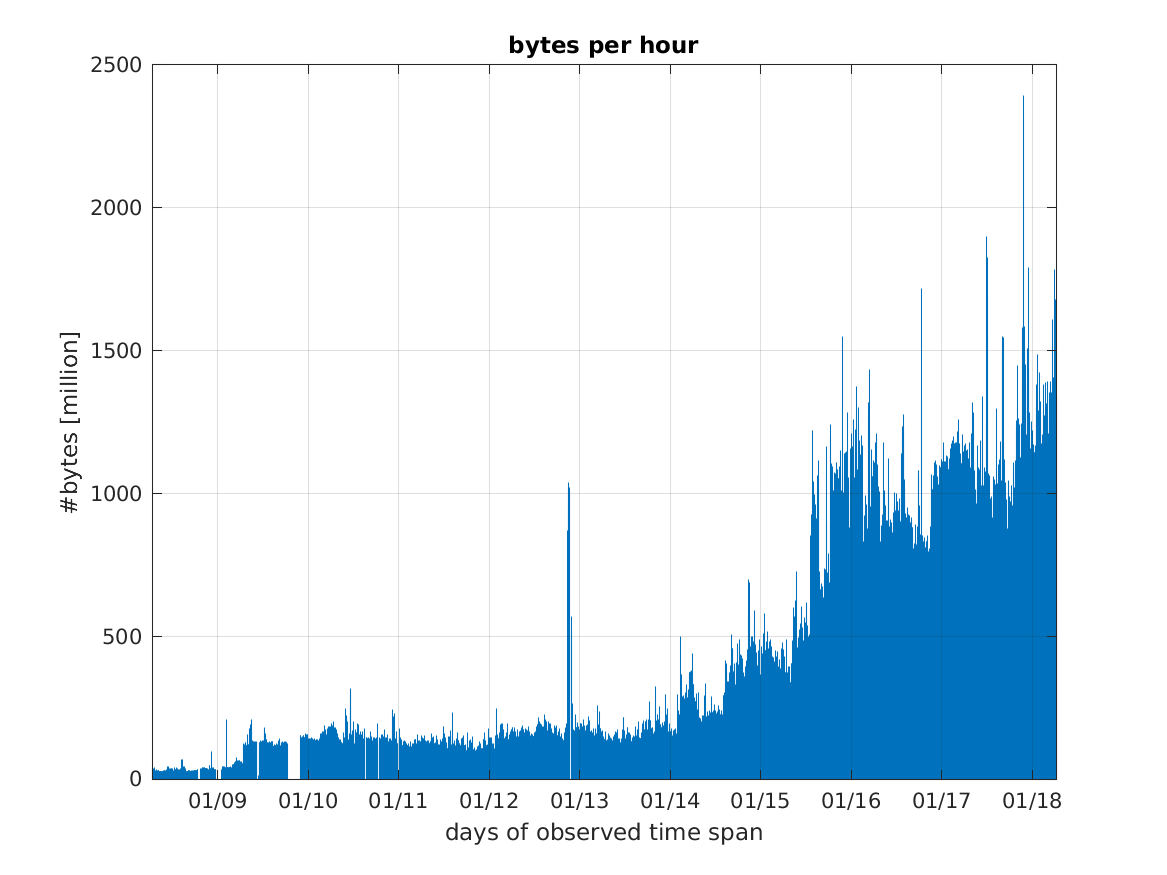
\includegraphics[width=\textwidth]{../exercise-3/plots/rep_10_2}
        \caption{Bytes per hour}
    \end{subfigure}
    \begin{subfigure}{.5\textwidth}
        \centering
        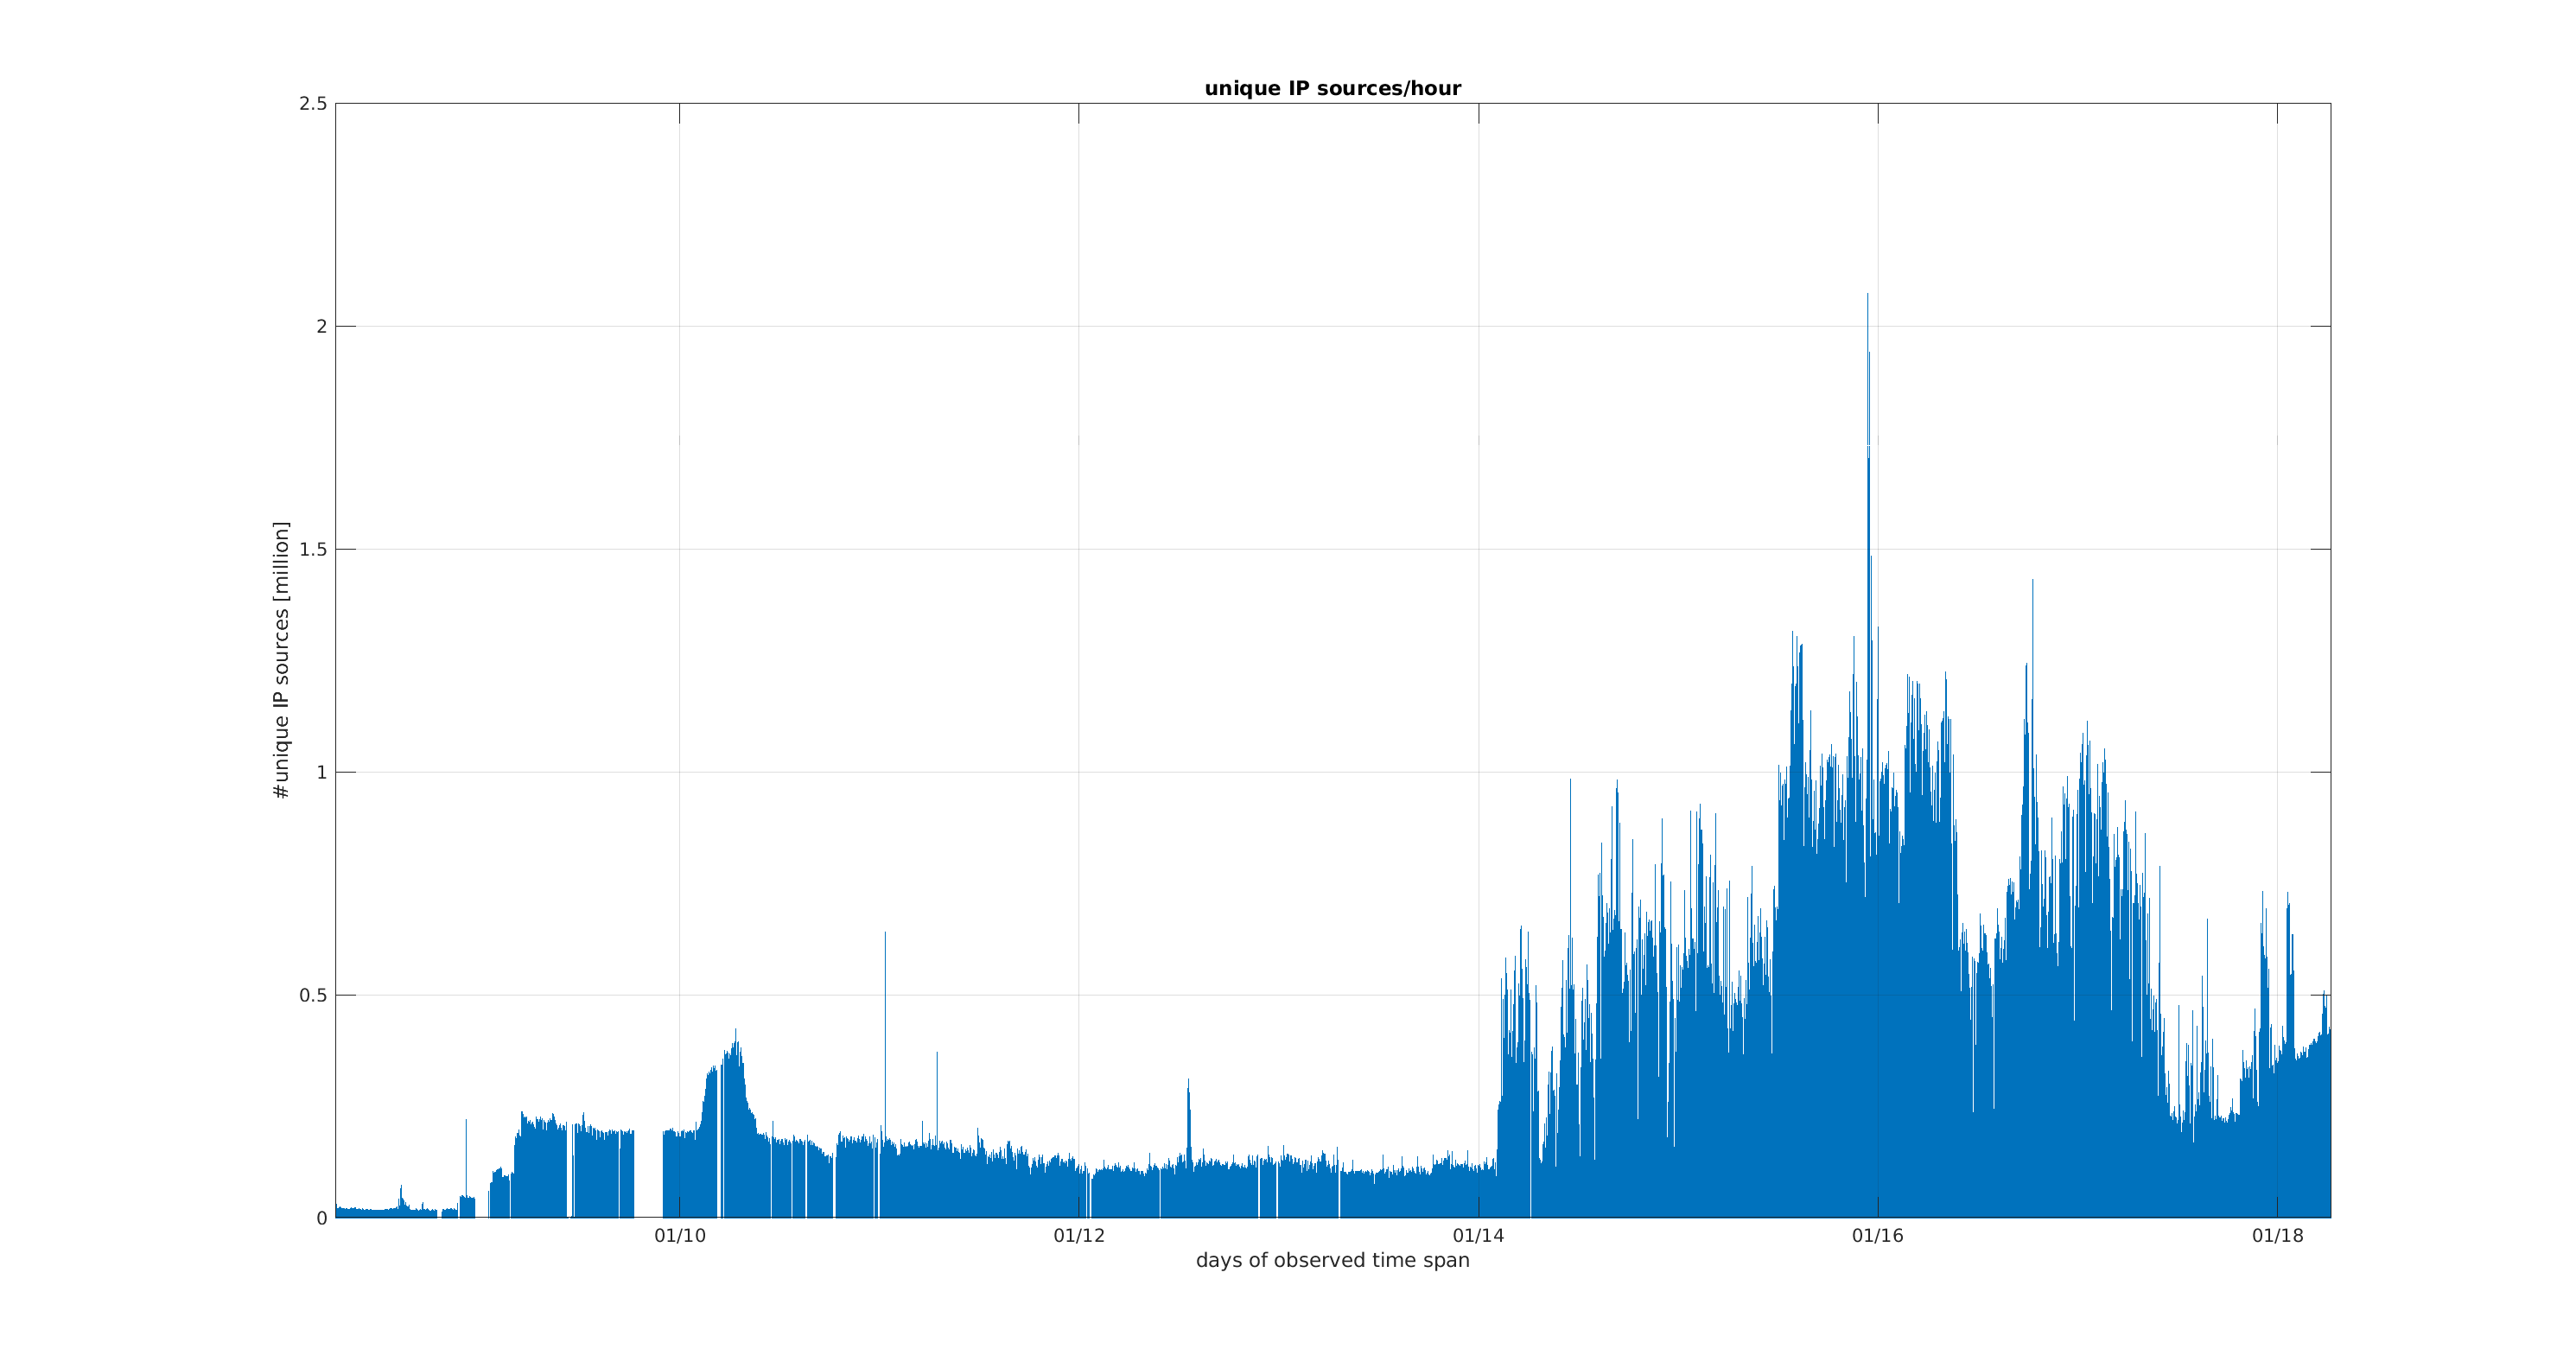
\includegraphics[width=\textwidth]{../exercise-3/plots/rep_10_3}
        \caption{IP sources per hour}
    \end{subfigure}
    \begin{subfigure}{.5\textwidth}
        \centering
        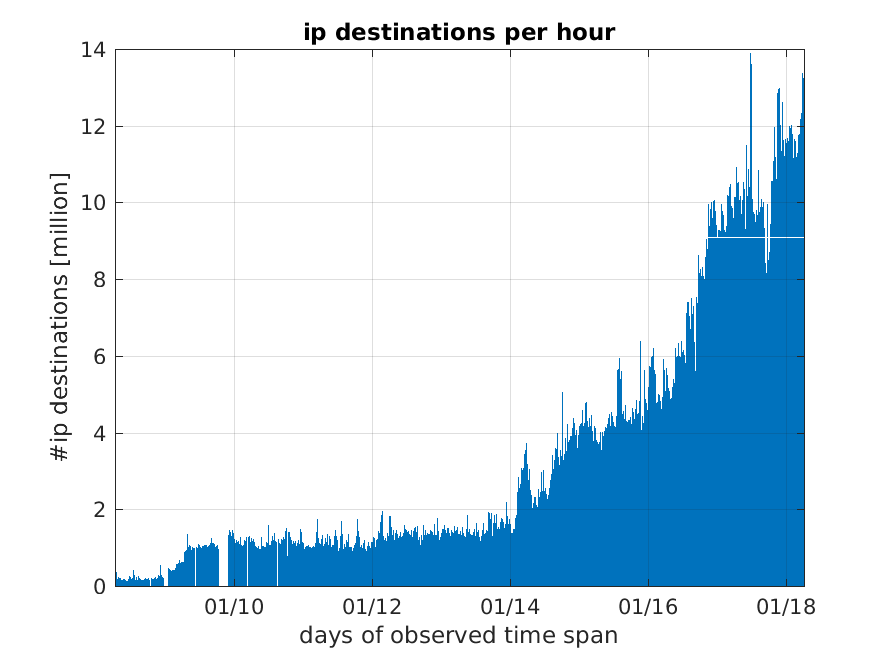
\includegraphics[width=\textwidth]{../exercise-3/plots/rep_10_4}
        \caption{IP destinations per hour}
    \end{subfigure}
    \caption{\label{figure:rep-10}}
\end{figure}

\paragraph{Optional}

Figure~\ref{figure:rep-10-optional} shows all signals from Figure~\ref{figure:rep-10} combined, normalized
and smoothed with a moving average filter.

\begin{figure}[h]
    \centering
    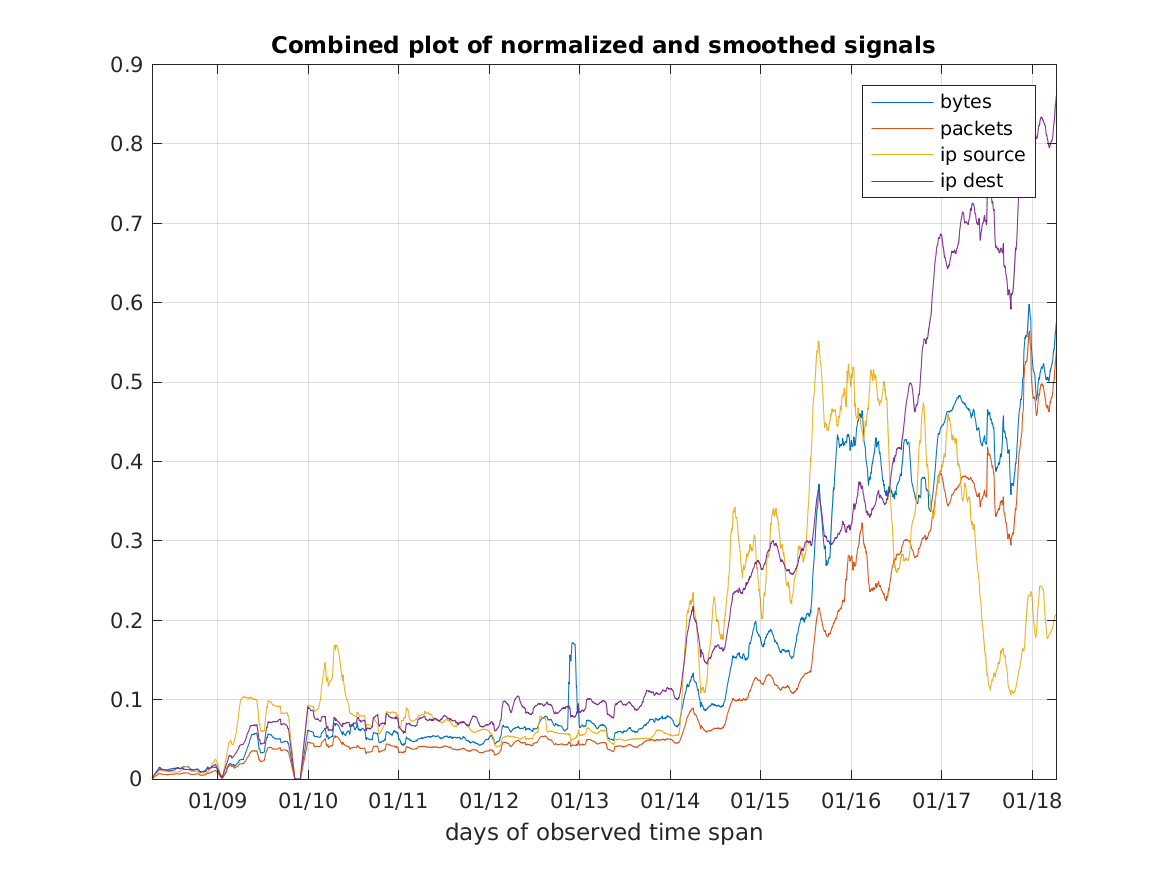
\includegraphics[width=\textwidth]{../exercise-3/plots/rep_10_optional}
    \caption{\label{figure:rep-10-optional} Combined, normalized and smoothed signals}
\end{figure}

\subsection{rep-11 \codelink{code:rep-11}}

The signal that shows the lower correlation to the other signals is \textbf{IP sources}. The minimum
linear correlation coefficient is \textbf{0.588568} between the signals \textbf{IP sources} and
\textbf{IP destinations}. See Table~\ref{table:rep-11} for the raw data.

\begin{table}[H]
    \centering
    \begin{tabular}{l|c|c|c|c}
                & Bytes  & Packets& IP src    & IP dst    \\
        \hline
        Bytes   & 1      & 0.9655 & 0.7203 & 0.9340 \\
        Packets & 0.9655 & 1      & 0.6105 & 0.9732 \\
        IP src     & 0.7203 & 0.6105 & 1      & 0.5886 \\
        IP dst     & 0.9340 & 0.9732 & 0.5886 & 1      \\
    \end{tabular}
    \caption{\label{table:rep-11} Correlation coefficients between signals}
\end{table}

The reason for why the drop in unique IP sources does not cause a proportional drop in the other
signals, could be that many small attackers (botnets), that did not contribute a lot to the other
signals somehow stopped sending traffic.

\subsection{rep-12 \codelink{code:rep-12}}

The number of IP sources is bigger in average than the number of darkspace addresses
receiving packets. There are on average around ten times more IP sources than IP destinations.
This makes sense, because the darkspace is only a small part of the internet address-space, but
the IP sources are taken from the whole address-space.

\subsection{rep-13 \codelink{code:rep-13}}

The main peak in IP sources starts on 14-Dec-2015 and lasts until 16-Dec-2015. See Table~\ref{table:rep-13}
for the detailed data.

\begin{table}[H]
    \parbox{.5\linewidth}{
        \centering
        \begin{tabular}{c|r}
            Date & \# IP sources \\
            \hline
            14-Dec-2015 & 2075358.074306 \\
            15-Dec-2015 & 1704892.012500 \\
            16-Dec-2015 & 1942072.404167 \\
        \end{tabular}
        \caption{\label{table:rep-13} Detailed data for peak in IP sources}
    }
    \parbox{.5\linewidth}{
        \centering
        \begin{tabular}{c|r}
            Date & \# Bytes \\
            \hline
            14-Nov-2012& 870858582.136110 \\ 
            15-Nov-2012& 1009586335.331900 \\
            16-Nov-2012& 1038654926.456100 \\
            17-Nov-2012& 1021464983.022200 \\
            18-Nov-2012& 954193481.914190 \\ 
            20-Nov-2012& 1005163238.508500 \\
            21-Nov-2012& 1020526661.658000 \\
            22-Nov-2012& 989613880.615110  \\
        \end{tabular}
        \caption{\label{table:rep-13-optional} Detailed data for peak in Bytes}
    }
\end{table}

\paragraph{Optional \codelink{code:rep-13-optional}}

The main peak in Bytes starts on 14-Nov-2012 and lasts until 22-Nov-2012. Note that
on 19-Nov-2012 no data was available. See Table~\ref{table:rep-13-optional}
for the detailed data.

\subsection{rep-14 \codelink{code:rep-14}}

Table~\ref{table:rep-14-daily} gives statistics for the data from
\texttt{global\_last10years.csv}. Table~\ref{table:rep-14-hourly} gives
statistics for the data from \texttt{Feb2017\_gen.csv}.

\begin{table}[H]
    \centering
    \begin{tabular}{l|rrrr}
                & Sum & Mean & Median & StdDev \\
                \hline
        \# Packets [millions] &   146373.391 & 41.845 & 17.699 & 40.916 \\
        \# Bytes [millions]   &    2381.003 & 0.681 & 0.263 & 0.735 \\
        \# IP src [millions]     & 123.613 & 0.035 & 0.020 & 0.031 \\
        \# IP dst  [millions]    & 1150.796 & 0.329 & 0.142 & 0.330 \\
    \end{tabular}
    \caption{\label{table:rep-14-daily} Statistics for daily data}
\end{table}

\begin{table}[H]
    \centering
    \begin{tabular}{l|rrrr}
                & Sum & Mean & Median & StdDev \\
                \hline
        \# Packets [millions] &    76871.319 & 114.392 & 113.464 & 7.033 \\
        \# Bytes  [millions]  &    1272.998  &1.894 & 1.890 & 0.097      \\
        \# IP src  [millions]    & 59.651 & 0.089 & 0.091 & 0.018        \\
        \# IP dst   [millions]   & 619.875 & 0.922 & 0.931 & 0.070       \\
    \end{tabular}
    \caption{\label{table:rep-14-hourly} Statistics for hourly data}
\end{table}

\subsection{rep-15}

The values do not coincide. February 2017 seems to be a month that is not really representative for the
data collected over a span of 10 years.

\paragraph{Optional \codelink{code:rep-15-optional}}
Figure~\ref{figure:rep-15-optional} shows the boxplots for hourly and daily averaged data.

\begin{figure}[h]
    \centering
    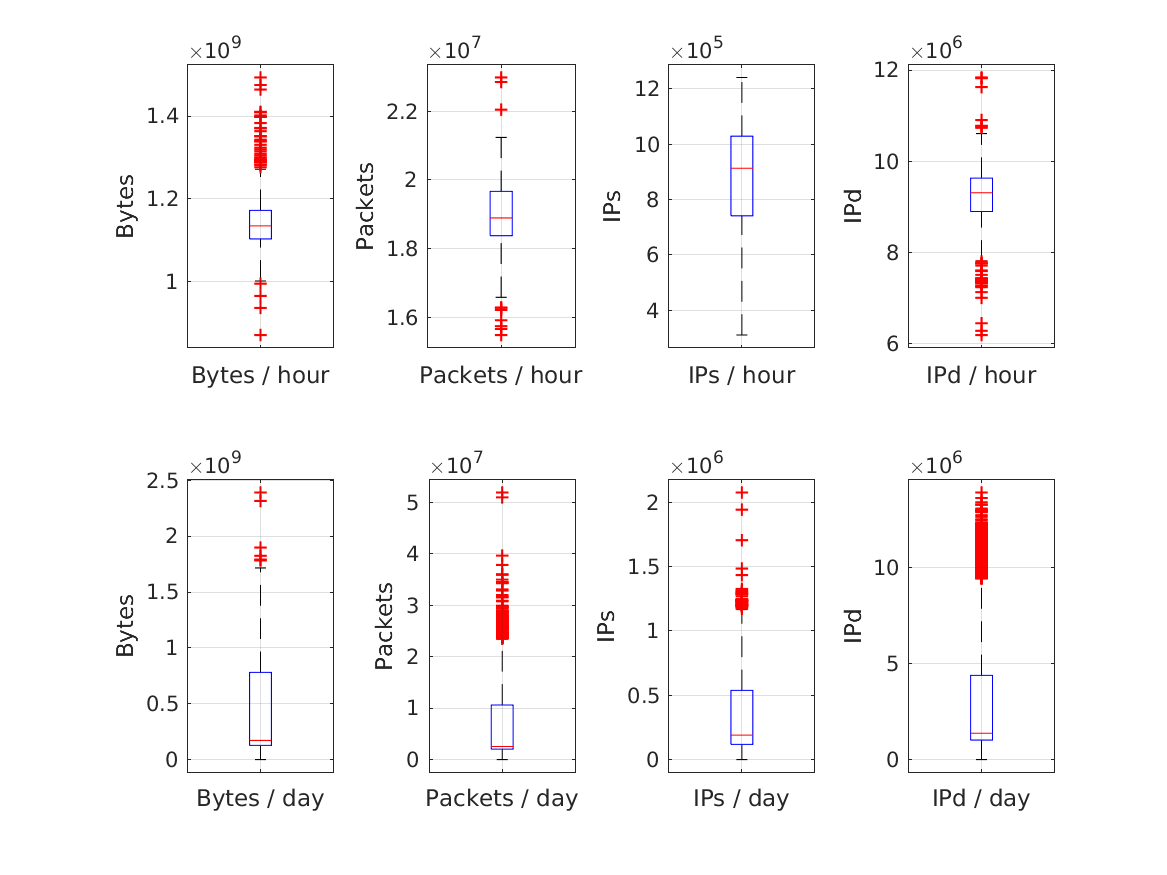
\includegraphics[width=\textwidth]{../exercise-3/plots/rep_15_optional}
    \caption{\label{figure:rep-15-optional} Boxplots for hourly and daily averaged data}
\end{figure}

A difference between the box plots for the hourly and daily data are the positions of
the medians in the plots. The medians in the daily averaged data show a clear tendency to
be in the vicinity of the first quartile, whereas the medians in the hourly averaged data
show no clear tendency.
A second noticeable difference are the outliers. All outliers in the daily averaged data are
above the whiskers, whereas the boxplots for the hourly averaged data show outliers below and
above the whiskers.

\subsection{rep-16}

We used \texttt{https://www.iana.org/assignments/protocol-numbers/protocol-numbers.xhtml} to look up the
protocol numbers.

\paragraph{Protocol 6 (TCP)}
The Transmission Control Protocol is a connection oriented, reliable protocol that is widely used.
A TCP connection is created by performing a three-way handshake (SYN, SYN/ACK, ACK). TCP uses
port numbers to address applications.

\paragraph{Protocol 1 (ICMP)}
The Internet Control Message Protocol is part of the IP specification and used to exchange status and
error messages concerning the IP protocol. ICMP is transported via IP. The popular \texttt{ping} and
\texttt{traceroute} programs are applications that make use of ICMP.

\paragraph{Protocol 17 (UDP)}
The User Datagram Protocol is a connectionless, unreliable protocol. UDP does not perform
a three-way handshake, but also uses port numbers to address applications.

\subsection{rep-17 \codelink{code:rep-17}}

Table~\ref{table:rep-17-packets} shows statistical information for Packets/hour grouped by protocol.
Table~\ref{table:rep-17-ips} shows statistical information for IP sources/hour grouped by protocol.
Table~\ref{table:rep-17-ipd} shows statistical information for IP destinations/hour grouped by protocol.

\begin{table}[H]
    \parbox{.45\linewidth}{
        \centering
        \begin{tabular}{l|ccc}
                & Mean  & Median & StdDev \\
                   \hline
            TCP    & 0.840 & 0.833  & 0.048 \\
            UDP    & 0.114 & 0.113  & 0.032 \\
            ICMP   & 0.043 & 0.054  & 0.026 \\
            Others & 0.004 & 0.004  & 0.001 \\
        \end{tabular}
        \caption{\label{table:rep-17-packets} Statistical information for Packets per hour}
    }
    \parbox{.1\linewidth}{}
    \parbox{.45\linewidth}{
        \centering
        \begin{tabular}{l|ccc}
                   & Mean  & Median & StdDev \\
                   \hline
            TCP    &   0.592 & 0.519  & 0.143  \\
            UDP    &   0.336 & 0.343  & 0.034  \\
            ICMP   &   0.175 & 0.225  & 0.106  \\
            Others &  -0.103 & -0.103 & 0.044  \\
        \end{tabular}
        \caption{\label{table:rep-17-ips} Statistical information for IP sources per hour}
    }
\end{table}

\begin{table}[H]
    \centering
    \begin{tabular}{l|ccc}
               & Mean  & Median & StdDev \\
               \hline
        TCP    &  0.890 & 0.883&  0.039   \\
        UDP    &  0.158 & 0.155&  0.045   \\
        ICMP   &  0.080 & 0.104&  0.048   \\
        Others &  -0.127&  -0.142&  0.042 \\
    \end{tabular}
    \caption{\label{table:rep-17-ipd} Statistical information for IP destinations per hour}
\end{table}

Figure~\ref{figure:rep-17} shows
boxplots for the data from \texttt{Feb2017\_proto.csv} separated by protocol and signal.

\begin{figure}[h]
    \begin{subfigure}{.5\textwidth}
        \centering
        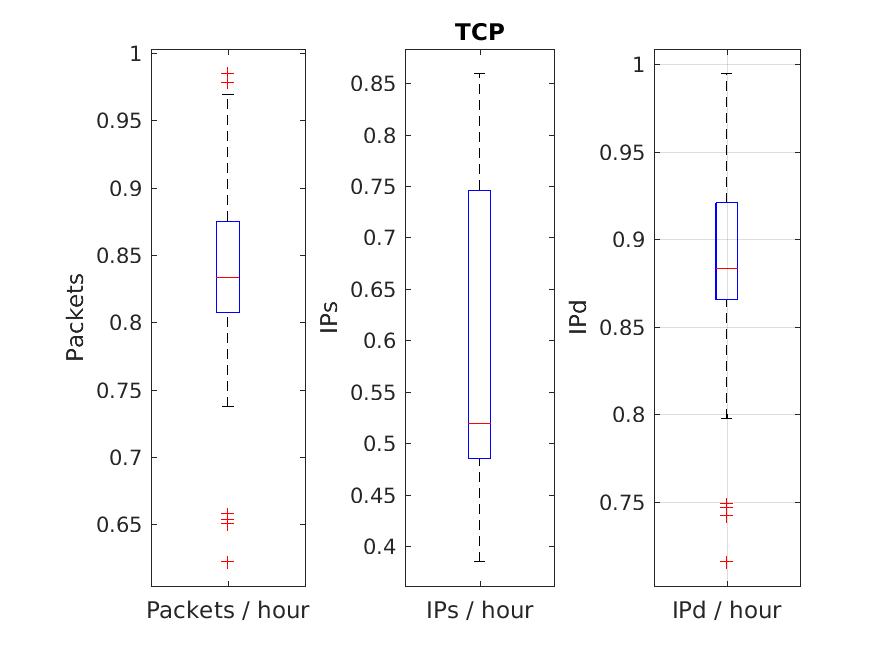
\includegraphics[width=0.7\textwidth]{../exercise-3/plots/rep_17_TCP}
        \caption{TCP}
    \end{subfigure}
    \begin{subfigure}{.5\textwidth}
        \centering
        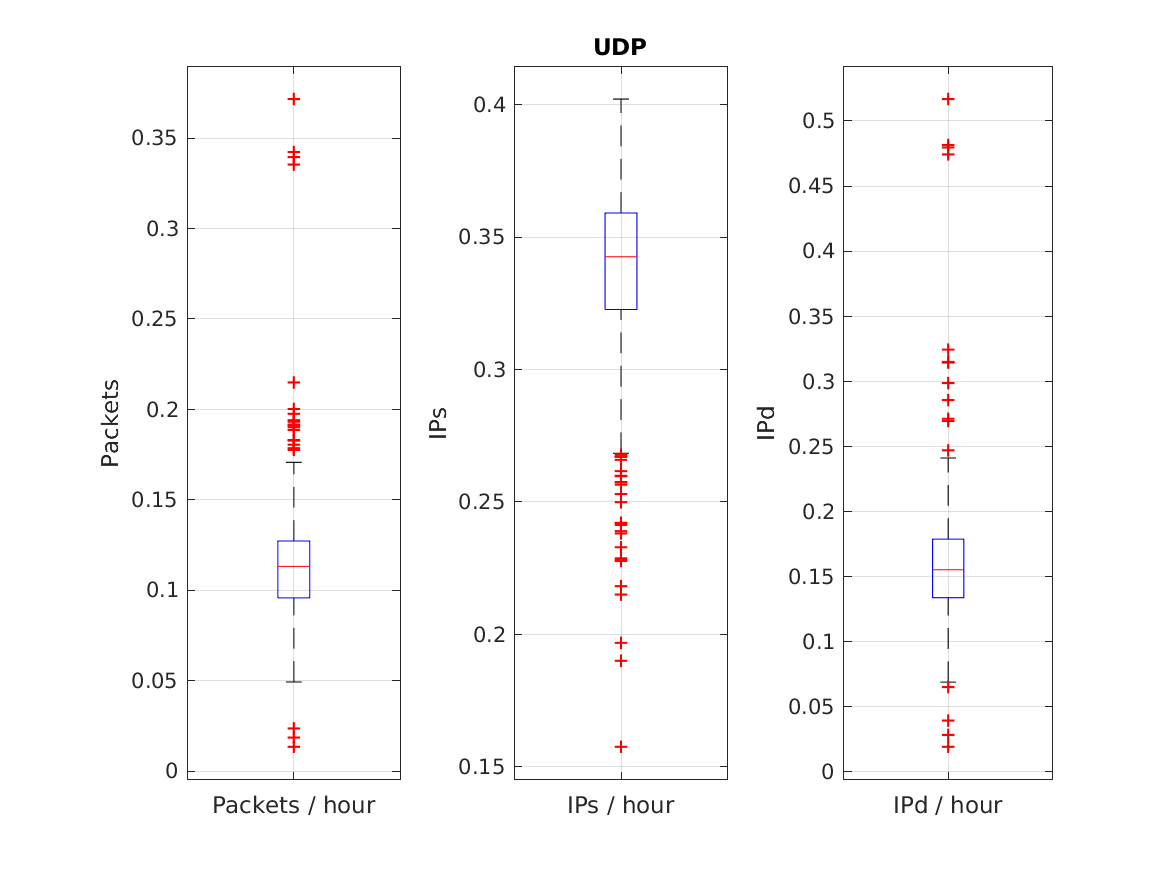
\includegraphics[width=0.7\textwidth]{../exercise-3/plots/rep_17_UDP}
        \caption{UDP}
    \end{subfigure}
    \begin{subfigure}{.5\textwidth}
        \centering
        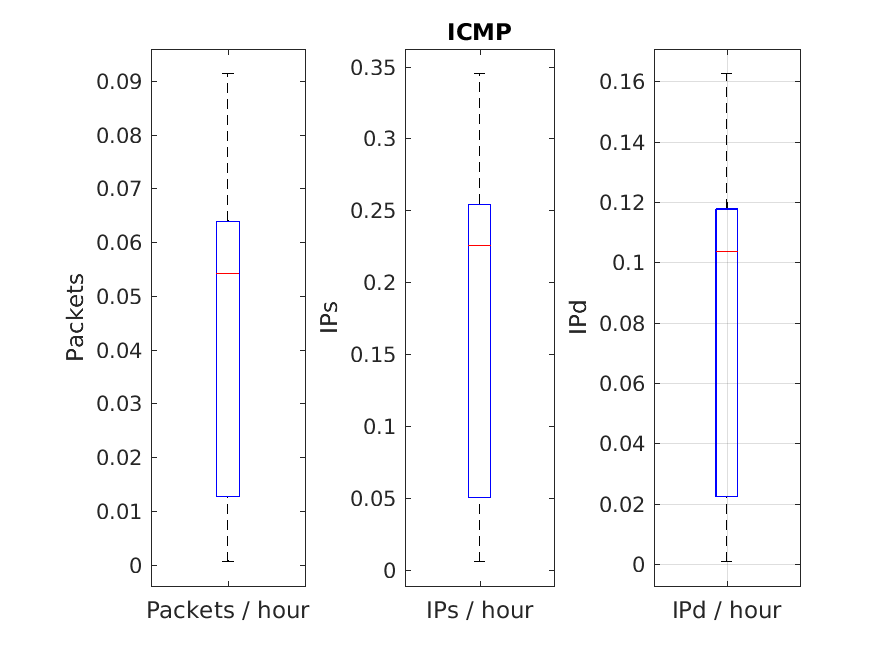
\includegraphics[width=0.7\textwidth]{../exercise-3/plots/rep_17_ICMP}
        \caption{ICMP}
    \end{subfigure}
    \begin{subfigure}{.5\textwidth}
        \centering
        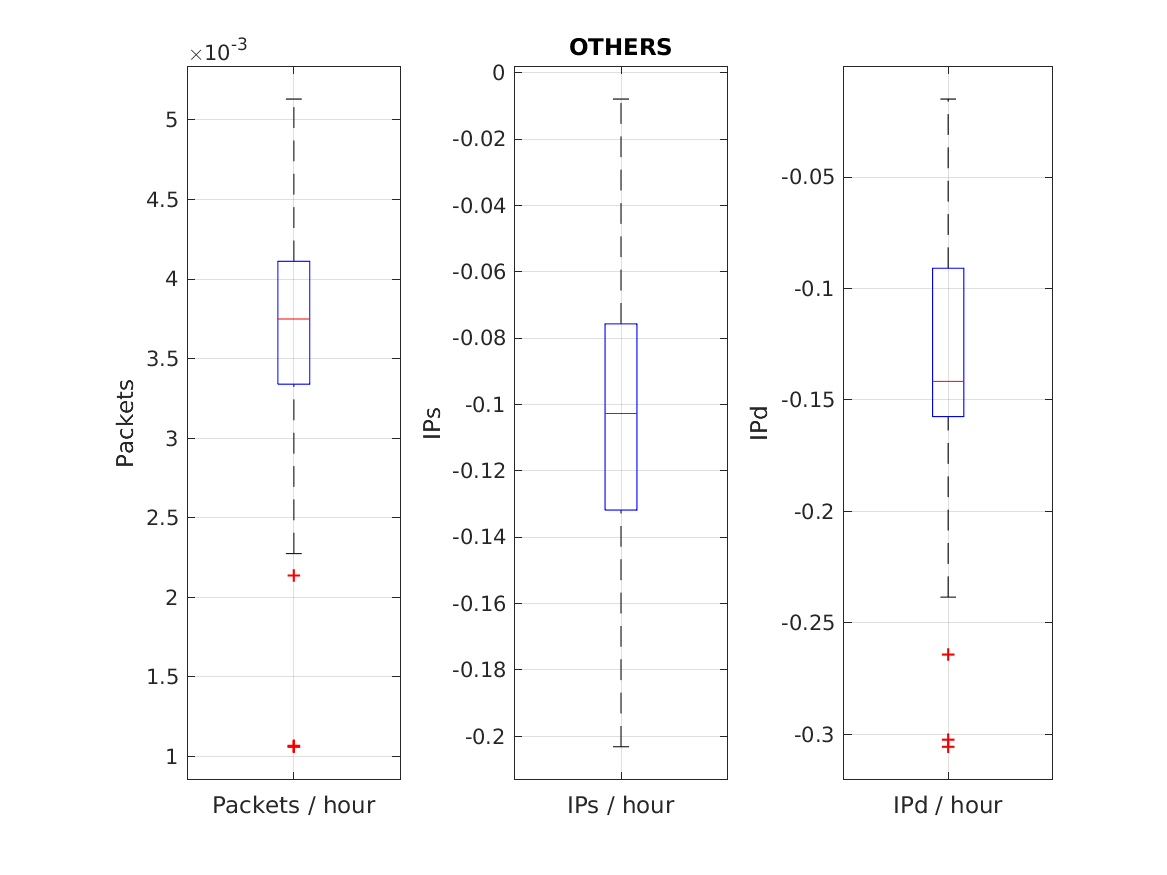
\includegraphics[width=0.7\textwidth]{../exercise-3/plots/rep_17_OTHERS}
        \caption{Others}
    \end{subfigure}
    \caption{\label{figure:rep-17} Boxplots separated by protocol and signal}
\end{figure}

\paragraph{Optional}

Figure~\ref{figure:rep-17-optional} shows the various scatter plots.

\begin{figure}[h]
    \begin{subfigure}{.5\textwidth}
        \centering
        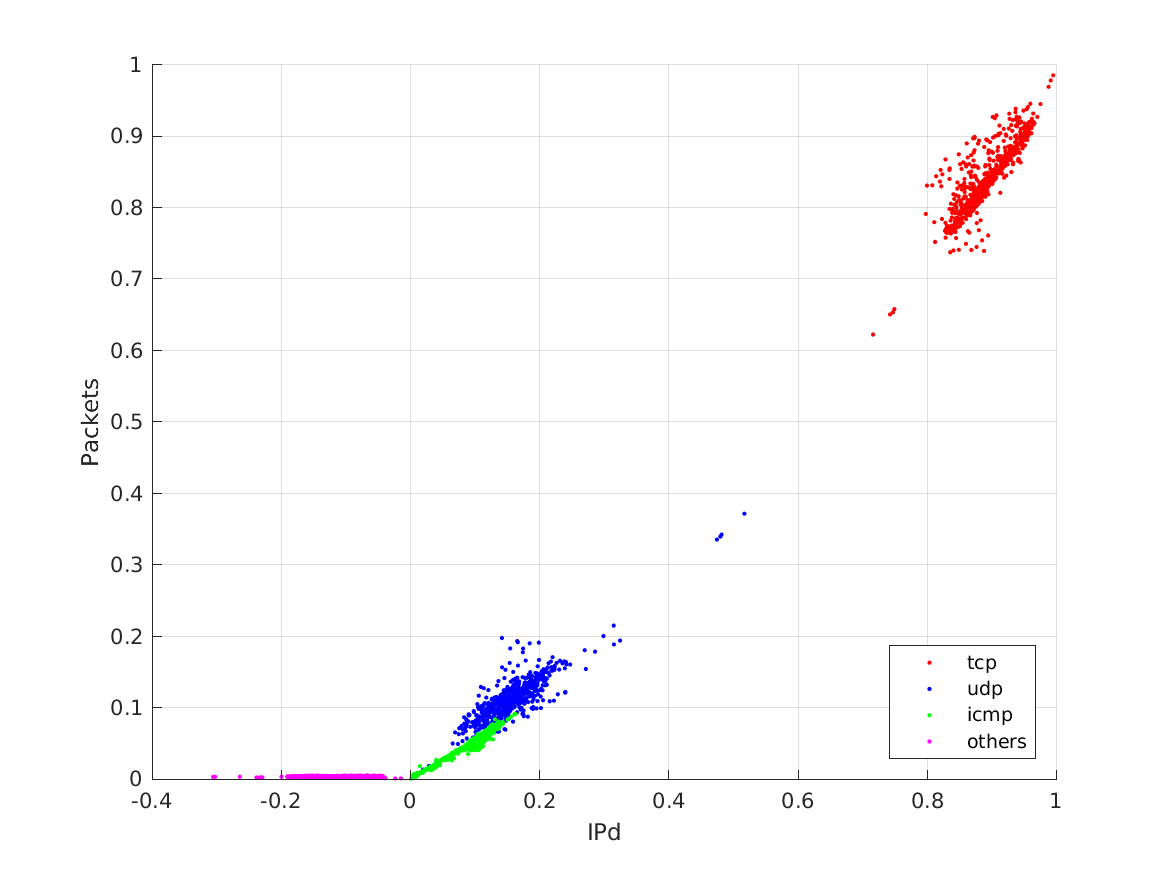
\includegraphics[width=\textwidth]{../exercise-3/plots/rep_17_optional_IPdPackets.png}
        \caption{Packets vs IP destinations}
    \end{subfigure}
    \begin{subfigure}{.5\textwidth}
        \centering
        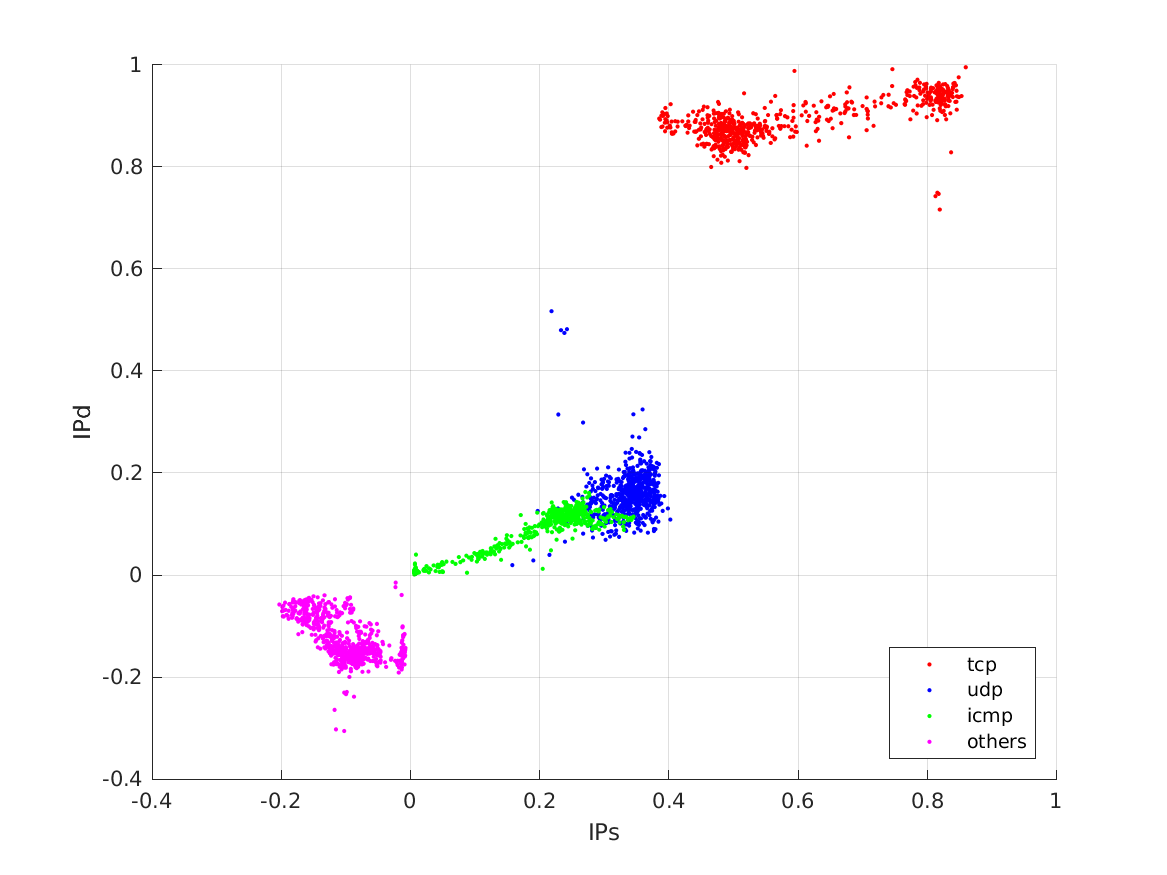
\includegraphics[width=\textwidth]{../exercise-3/plots/rep_17_optional_IPsIPd.png}
        \caption{IP destinations vs IP sources}
    \end{subfigure}
    \begin{subfigure}{.5\textwidth}
        \centering
        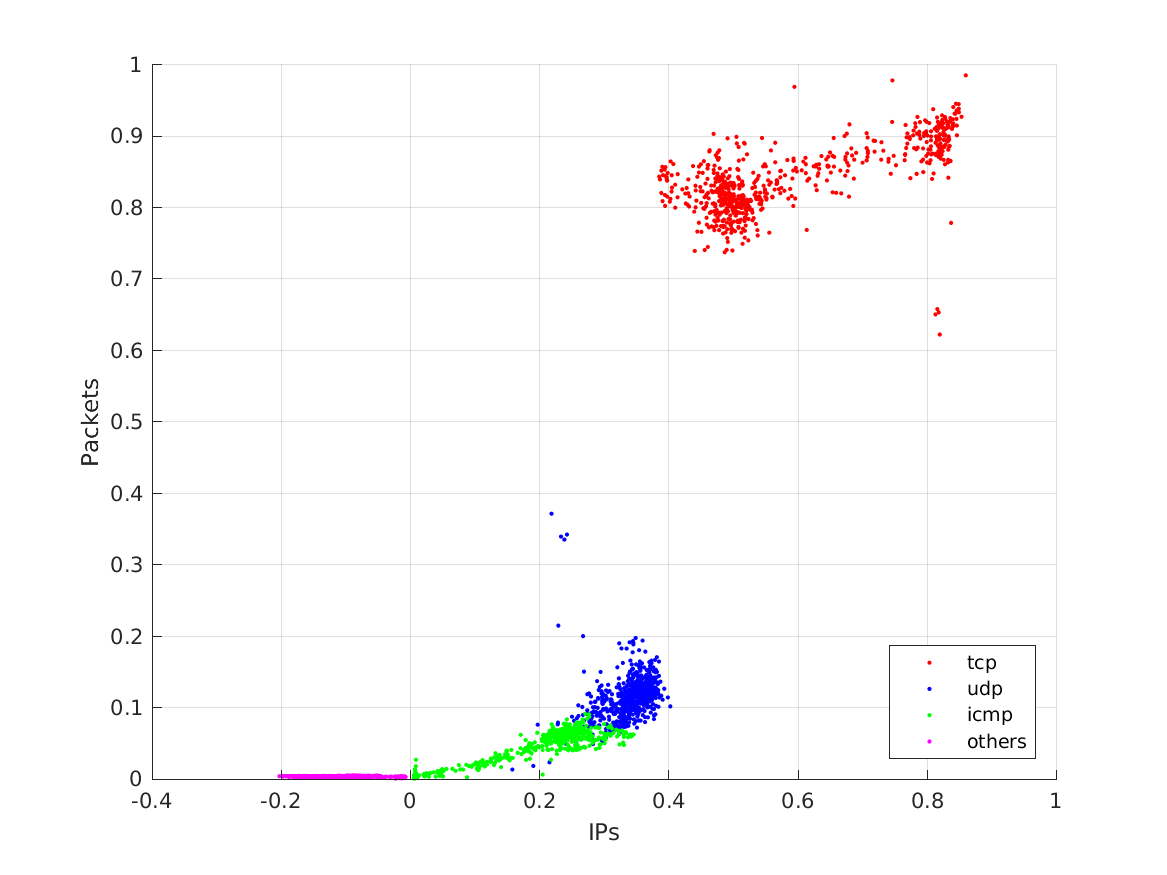
\includegraphics[width=\textwidth]{../exercise-3/plots/rep_17_optional_IPsPackets.png}
        \caption{Packets vs IP sources}
    \end{subfigure}
    \caption{\label{figure:rep-17-optional} Scatter plots}
\end{figure}

\subsection{rep-18}

We obtained negative values for unique IP sources and destinations for ``other'' protocols because, in
the combined data addresses are collapsed. The same address might get a TCP, a UDP and an ICMP packet, but
will only be counted once.

\subsection{rep-19 \codelink{code:rep-19}}

The four most used ports in descending order are port 23, port 22, port 445 and port 80.
Table~\ref{table:rep-19-absolute} shows statistical information in absolute values for the
four most used ports in the data file. Table~\ref{table:rep-19-percentage} shows the statistical
information in percentages.

\paragraph{Port 23 (Telnet)}
We see traffic to this port in the darkspace, because many devices on the internet have a
telnet daemon listening on port 23 - often with minimal password protection. The connection
attempts to port 23 are part of automated scanning for open telnet ports.

\paragraph{Port 22 (SSH)}
We see traffic to this port in the darkspace, because many host on the internet have an
SSH daemon listening on port 22. The connection attempts to port 22 are part of automated scanning
for open SSH ports - often followed by a dictionary based password guessing attack.

\paragraph{Port 445 (Microsoft Directory Service)}
We see traffic to this port in the darkspace, because the ``Microsoft Directory Service'' 

\paragraph{Port 80 (HTTP)}
We see traffic to this port, because many hosts on the internet have a webserver running
on port 80. The connection attempts to port 80 are part of automated scanning for webservers.

\begin{table}[H]
    \centering
    \begin{tabular}{l|cccc}
        & Port 23 & port 22 & Port  445 & Port 80 \\
        \hline
        Mean &  0.627 & 0.049 & 0.026 & 0.015 \\
        StdDev &  0.113 & 0.025 & 0.005 & 0.010 \\
    \end{tabular}
    \caption{\label{table:rep-19-absolute} Statistical information for TCP packets [in million]}
\end{table}

\begin{table}[H]
    \centering
    \begin{tabular}{l|cccc}
        & Port 23 & port 22 & Port  445 & Port 80 \\
        \hline
        Mean &   39.7 & 3.1 & 1.6 & 0.9  \\
        StdDev & 7.3  & 1.5 & 0.3 & 0.6   \\
    \end{tabular}
    \caption{\label{table:rep-19-percentage} Statistical information for TCP packets [in percent]}
\end{table}

\subsection{rep-20 \codelink{code:rep-20}}
Figure~\ref{figure:rep-20} shows the data for the ports 445 and 502. Data associated with port 445 is
the data with the lowest relative difference between mean and median, data associated with port 502 is
the data with the highest relative difference between mean and median.

\begin{figure}[h]
    \centering
    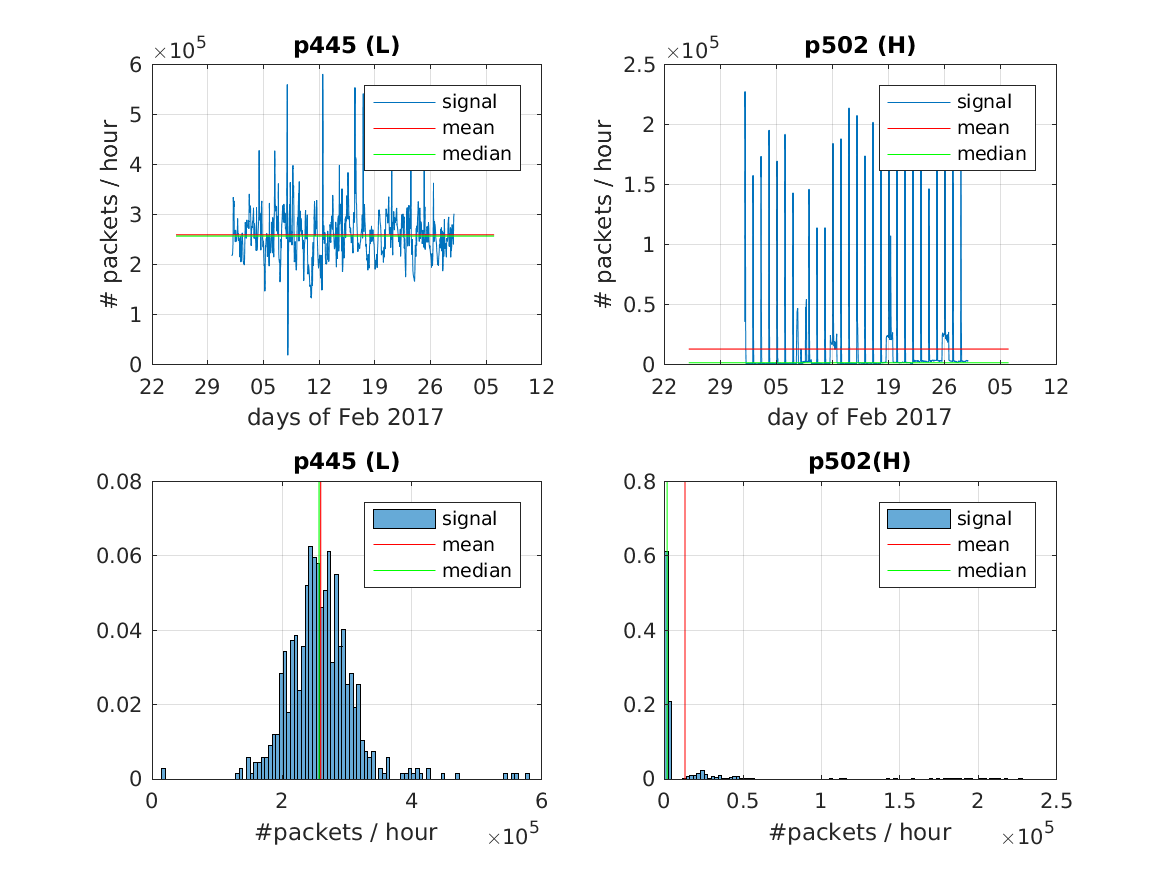
\includegraphics[width=\textwidth]{../exercise-3/plots/rep_20.png}
    \caption{\label{figure:rep-20} Data with highest and lowest relative difference between mean and median}
\end{figure}


\fxerror{Wording - fill in!}
The mean/median better represents the average value of a dataset. why? skewness with regard to distributions
An example for a distribution where the mean or the 

\subsection{rep-21 \codelink{code:rep-21}}

Figure~\ref{figure:rep-21-timeseries} shows the time series plot for the number of packets per hour and the
number of unique IP sources per hour.
Figure~\ref{figure:rep-21-fft} shows the amplitude spectra for the number of packets per hour and the
number of unique IP sources per hour.

\begin{figure}[h]
    \centering
    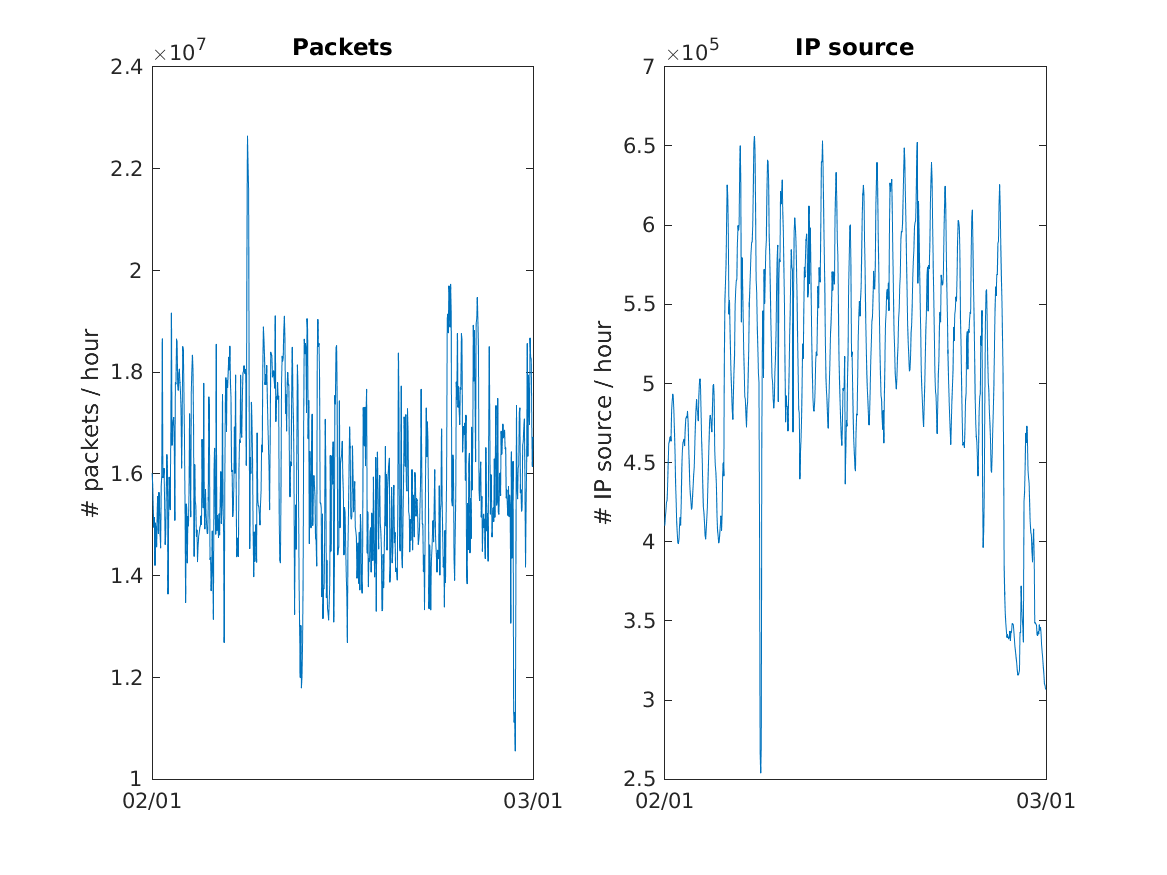
\includegraphics[width=\textwidth]{../exercise-3/plots/rep_21_a}
    \caption{\label{figure:rep-21-timeseries} Time series plots for TCP for February 2017}
\end{figure}

\begin{figure}[h]
    \centering
    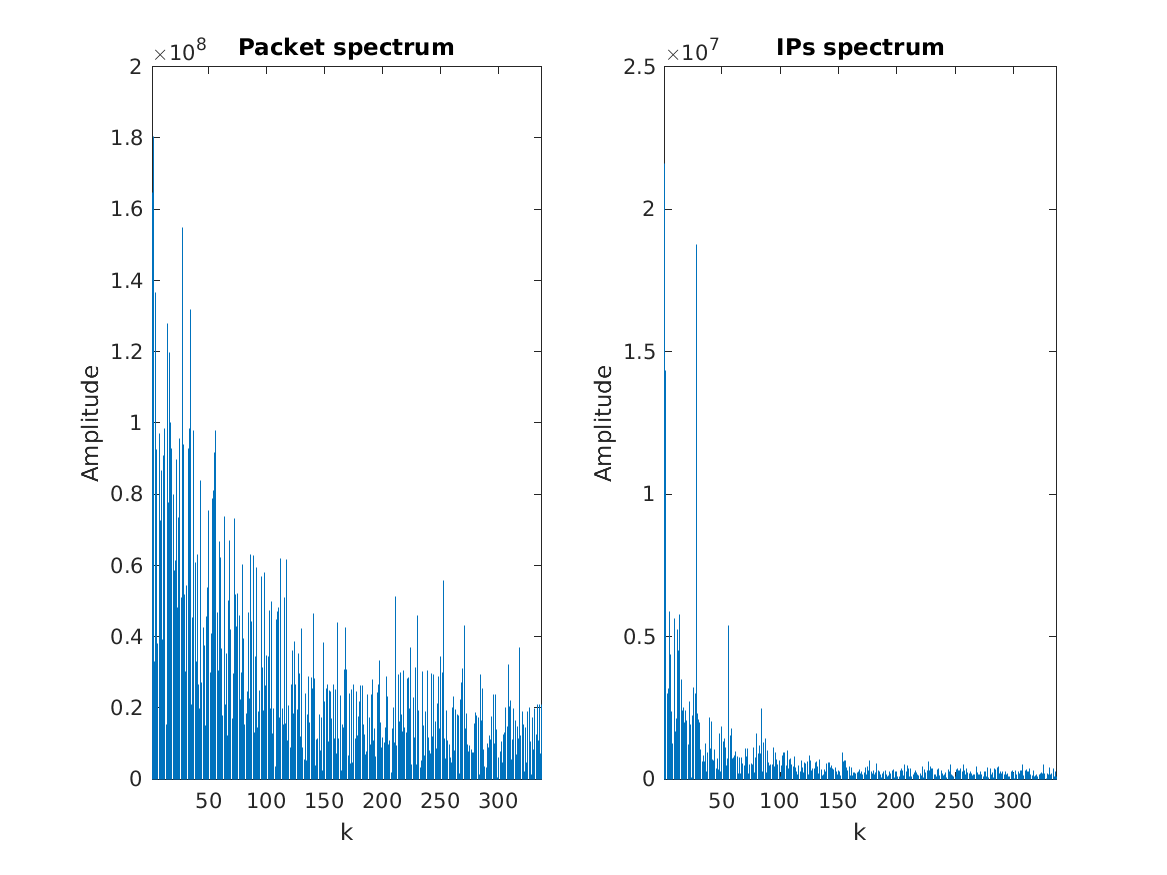
\includegraphics[width=\textwidth]{../exercise-3/plots/rep_21_b}
    \caption{\label{figure:rep-21-fft} Amplitude spectra for TCP for February 2017}
\end{figure}

\paragraph{Periodicity}
Table~\ref{table:rep-21-max-fft} shows the maximum FFT value and associated information for Packets
per hour and unique IP sources per hour.
Table~\ref{table:rep-21-fft-packets} shows further temporal patterns found in the signal for Packets
per hour.
Table~\ref{table:rep-21-fft-ips} shows further temporal patterns found in the signal for unique IP
sources per hour.

\begin{table}[h]
    \centering
    \begin{tabular}{l|r|r|r|r}
                       & FFT maximum value & k & Period (days) & Period (hours) \\
        \hline
        Packets / hour & 180308368.771 & 2 & 14 & 336 \\
        IP src / hour & 21586333.529 & 1 & 28 & 672 \\
    \end{tabular}
    \caption{\label{table:rep-21-max-fft} Maximum FFT value and futher information}
\end{table}

\begin{table}[H]
    \centering
    \begin{tabular}{l|r|r|r}
        FFT maximum value & Period (days) & Period (hours) & Comment \\
        \hline
        1.8031e+08 & 0.0418 & 1.0030 & Hourly pattern \\
        1.6480e+08 & 28 & 672 & Fundamental frequency \\
        1.6480e+08 & 0.0417 & 1.0015 & Another hourly pattern \\
        1.5489e+08 & 1.0370 & 24.8889 & Daily pattern \\
        1.5489e+08 & 0.0434 & 1.0419 & Another hourly pattern \\
        1.3649e+08 & 7 & 168 & Weekly pattern \\
        1.3649e+08 & 0.0419 & 1.0060 &  Another hourly pattern \\
    \end{tabular}
    \caption{\label{table:rep-21-fft-packets} Temporal patterns in Packets per hour}
\end{table}

\begin{table}[H]
    \centering
    \begin{tabular}{l|r|r|r}
        FFT maximum value & Period (days) & Period (hours) & Comment \\
        \hline
        2.1586e+07 & 0.0417 & 1.0015 & Hourly pattern \\
        1.8748e+07 & 1 & 24 & Daily pattern \\
        1.8748e+07 & 0.0435 &  1.0435 & Another hourly pattern \\
        1.4339e+07 & 14 &  336 & Bi-weekly pattern \\
        1.4339e+07 & 0.0418&  1.0030 & Another hourly pattern \\
    \end{tabular}
    \caption{\label{table:rep-21-fft-ips} Temporal patterns in unique IP sources per hour}
\end{table}

\subsection{rep-22 \codelink{code:rep-22}}

Figure~\ref{figure:rep-22} shows an average day for the number of packets per hour and the number of
unique IP sources per hour for February 2017.

\begin{figure}[h]
    \begin{subfigure}{.5\textwidth}
        \centering
        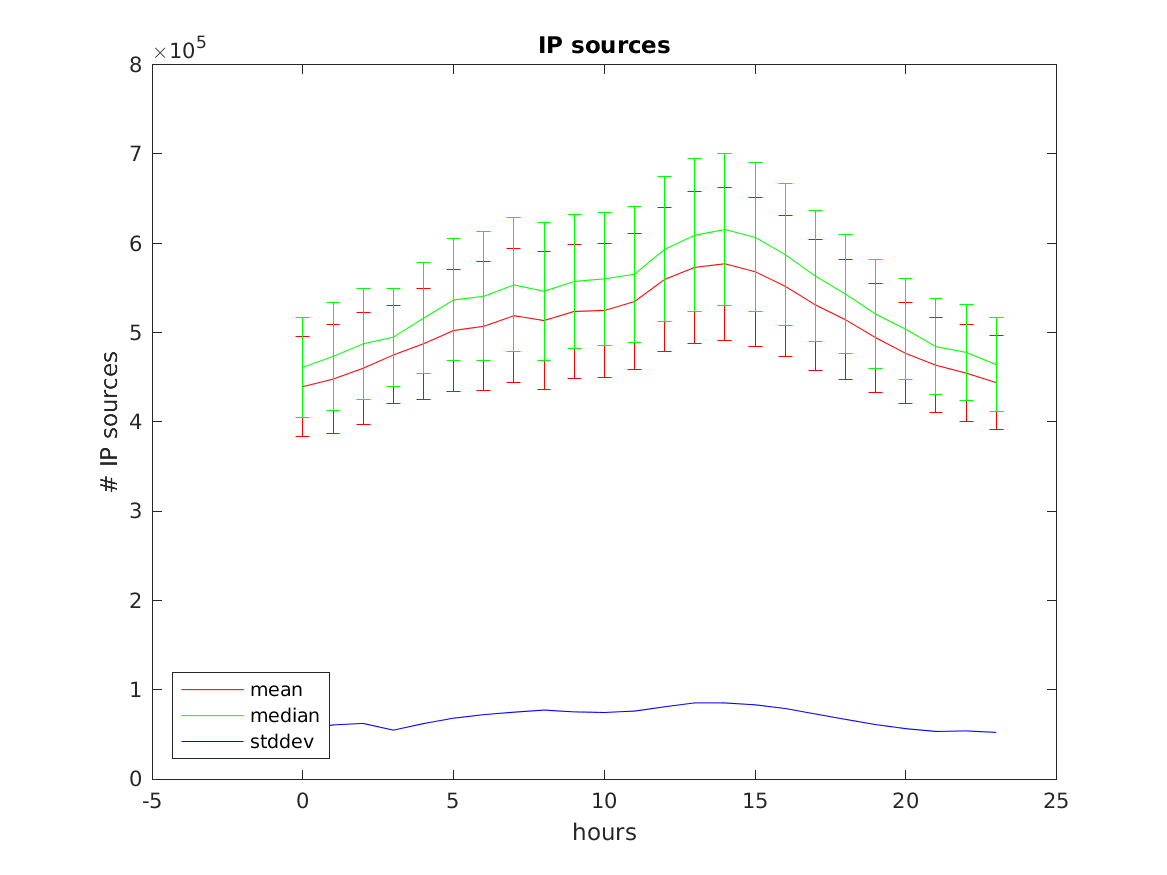
\includegraphics[width=\textwidth]{../exercise-3/plots/rep_22_ip_s}
        \caption{Average day for IP sources per hour}
    \end{subfigure}
    \begin{subfigure}{.5\textwidth}
        \centering
        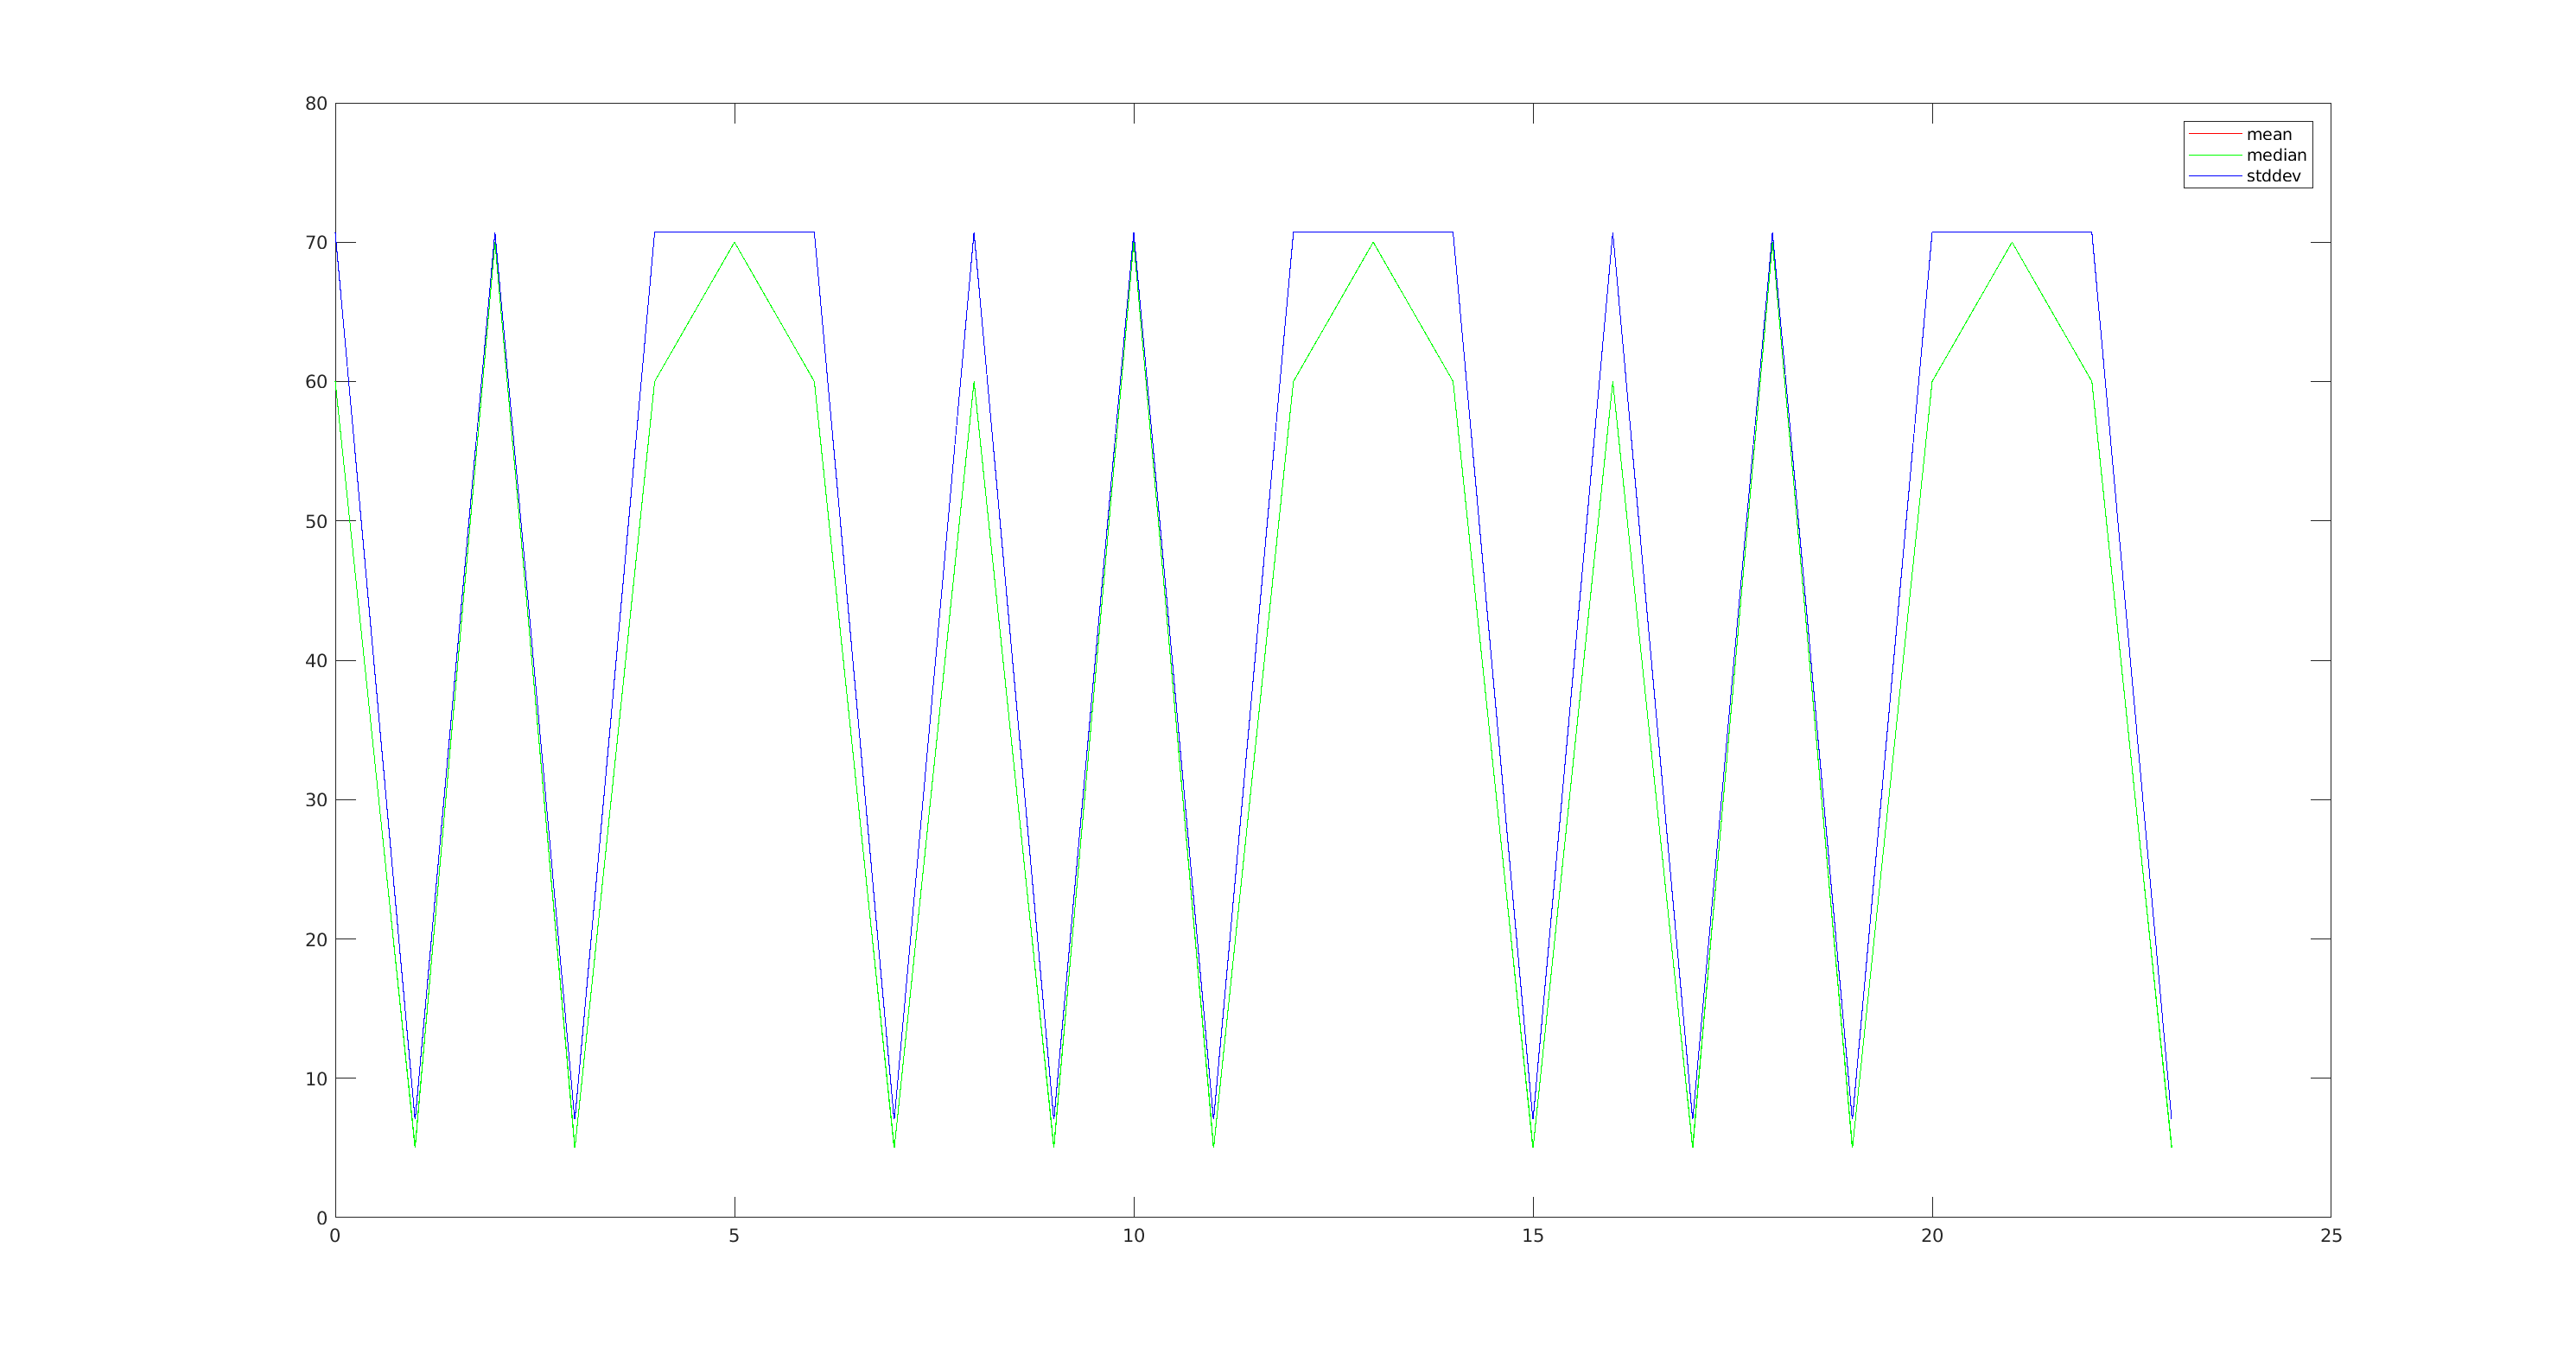
\includegraphics[width=\textwidth]{../exercise-3/plots/rep_22_packets}
        \caption{Average day for packets per hour}
    \end{subfigure}
    \caption{\label{figure:rep-22} Average days}
\end{figure}

\subsection{rep-23 \codelink{code:rep-22}} % NOTE: codelink is correct!

Table~\ref{table:rep-23} shows the correlation coefficients between the averaged signals for
Packets per hour and unique IP sources per hour.

\begin{table}[H]
    \centering
    \begin{tabular}{l|c}
        & Correlation coefficient \\
        \hline
        Mean & 0.0348 \\
        Median & 0.0485 \\
    \end{tabular}
    \caption{\label{table:rep-23} Correlation coefficients between Packets per hour and
    unique IP sources per hour}
\end{table}

When averaging with the median the correlation coefficient of the signals is slightly higher.
But the signals are not correlated. For the averaged signal for unique IP sources per hour
a prominent peak at around 2 pm can be observed. For the averaged signal of Packets per hour no
such prominent peak exists.

\FloatBarrier
\section{Lab Exercise 4}

\subsection{rep-24}

We converted the flowrecords into a CSV file using the command shown in Listing~\ref{listing:flow-to-csv}.

\begin{lstlisting}[label=listing:flow-to-csv,language=bash,caption={Command used to obtain CSV file}]
team02@pc01:~$ rwcut --num-recs=200000 --delimited=, \
    --fields=sIP,dIP,sPort,dPort,protocol,flags,ttl,bytes \
    ~/workfiles/team02.flowrecord.rw > team02_flowrecord.csv
\end{lstlisting}

\subsection{rep-25}

Table~\ref{table:rep-25-src} shows the three most frequent destination ports.
Table~\ref{table:rep-25-dst} shows the three most frequent source ports.
Table~\ref{table:rep-25-proto} shows all used protocols.

\begin{table}[H]
    \parbox{.45\linewidth}{
        \centering
        \begin{tabular}{l|r}
            Port & Rate of appearance (\%) \\
            \hline
            80 & 21.6 \\
            0 & 3.8 \\
            25565 & 1.6 \\
        \end{tabular}
        \caption{\label{table:rep-25-src} Three most frequent source ports}
    }
    \parbox{.45\linewidth}{
        \centering
        \begin{tabular}{l|r}
            Port & Rate of appearance (\%) \\
            \hline
            445 & 41.0 \\
            10320 & 9.6 \\
            3072 & 2.8 \\
        \end{tabular}
        \caption{\label{table:rep-25-dst} Three most frequent destination ports}
    }
\end{table}

\begin{table}[h]
    \centering
    \begin{tabular}{l|r}
        Protocol & Rate of appearance (\%) \\
        \hline
        TCP (6) & 81.5 \\
        UDP (17) & 15.1 \\
        ICMP (1) & 3.4 \\
        IPv6 (41) & 0.1 \\
        GRE (47) & 0.0 \\
    \end{tabular}
    \caption{\label{table:rep-25-proto} All used protocols}
\end{table}

\subsection{rep-26}

The rate of appearance concering the used protocols was roughly what we expected it to be. Port
445 as the top most used destination port was also no big surprise, but ports 10320 and 3072 where
somewhat surprising, because as far as we know no popular applications use these two ports.
Interesting to note are the two top most source ports 80 and 0. These ports are probably used to
bypass not properly configured firewalls.

\subsection{rep-27}

Figure~\ref{figure:rep-27} shows the TTL frequency distribution. Note the two peaks around a
TTL of 45 and a TTL of 107.

\fxerror{Explain!}

\begin{figure}[h]
    \centering
    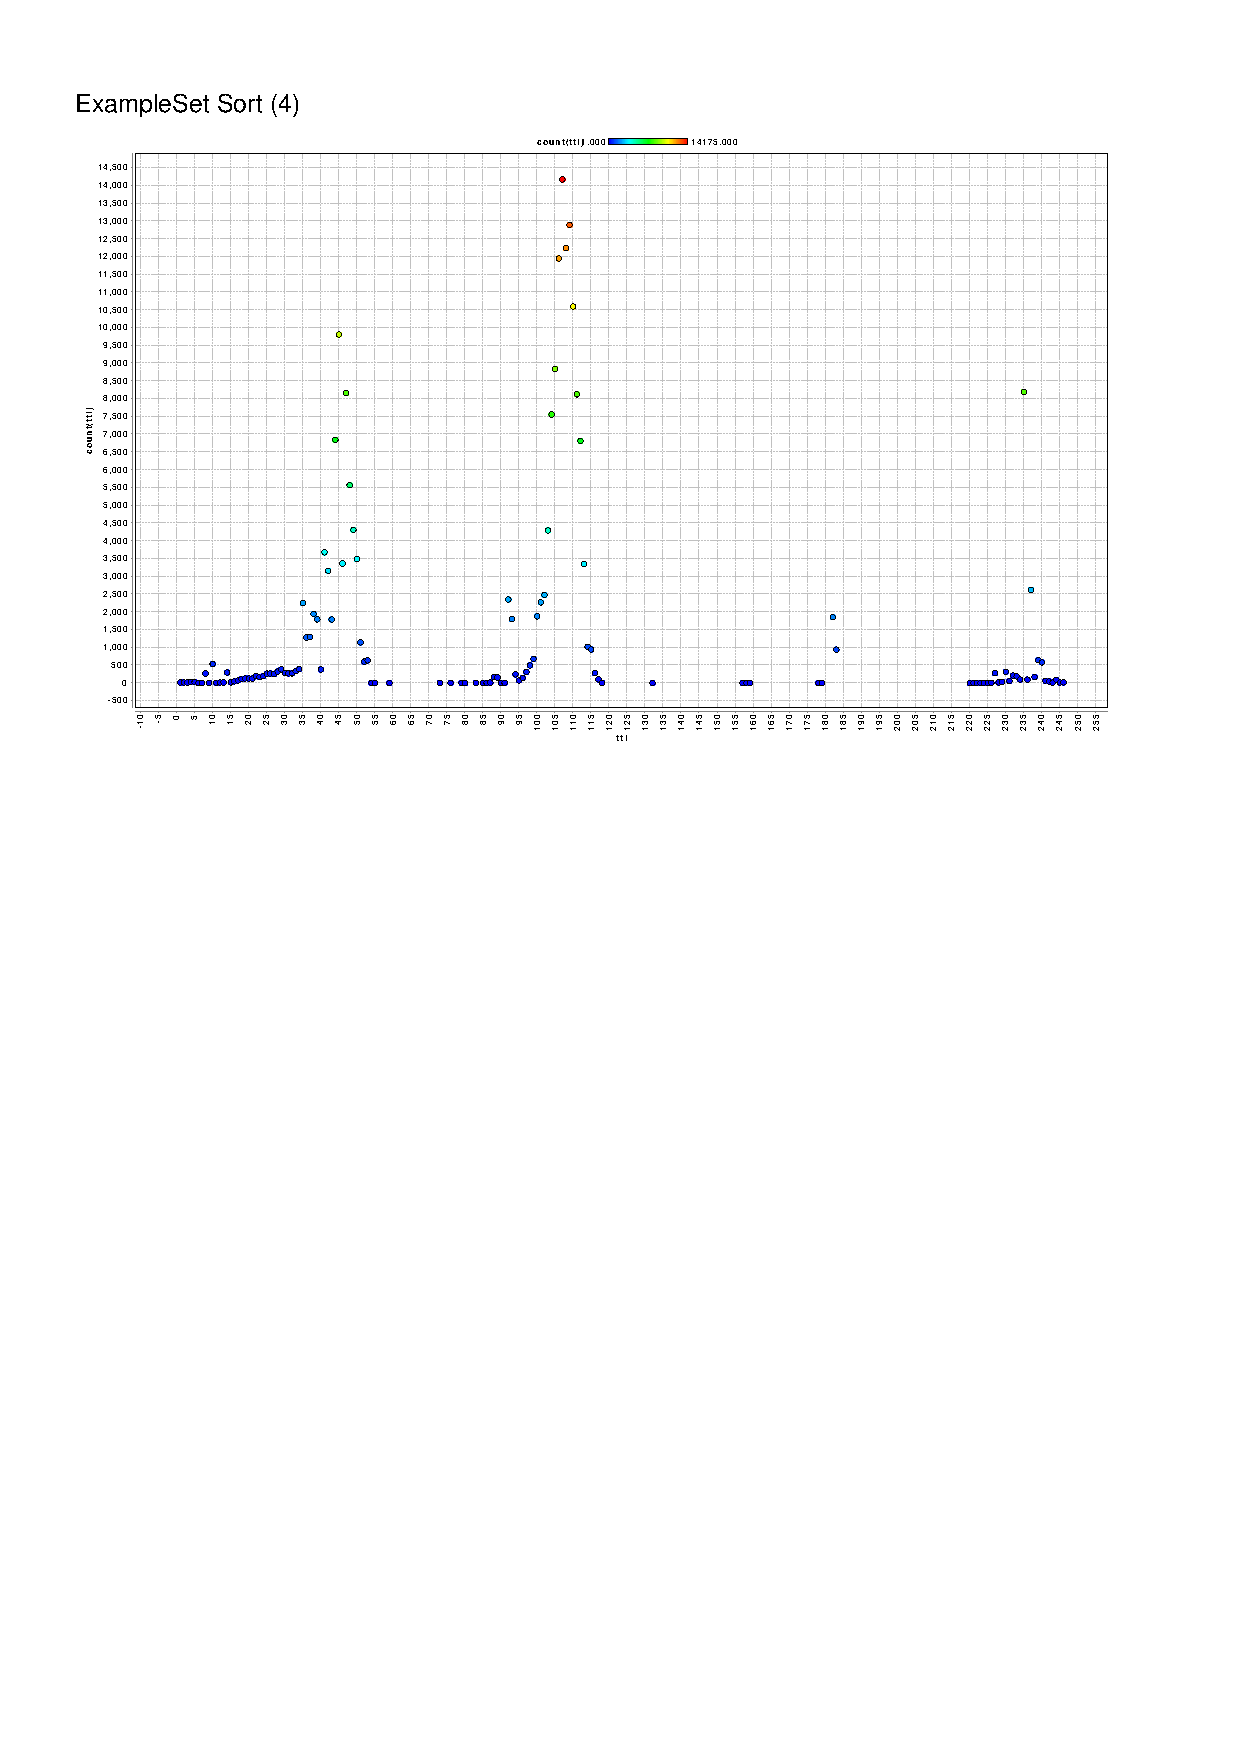
\includegraphics[clip, trim=1cm 17cm 2cm 2cm, width=1.00\textwidth]{../exercise-4/ttl.pdf}
    \caption{\label{figure:rep-27} TTL frequency distribution}
\end{figure}

\subsection{rep-28}

The most recurring IP source in our dataset is the IP address \texttt{236.196.32.152}.
It is exclusively using port \texttt{80} as a destination port and hitting ports \texttt{3072}
and \texttt{1024} across a range of IP destinations. The source is performing a horizontal port scans
for ports 3072 and 1024.

\subsection{rep-29}

To arrive at the desired data we performed some aggregation and filtering instead of
inspecting the scatter plot. The source IP that is connecting to the maximum number of
different ports is \texttt{72.99.52.73}.
Figure~\ref{figure:rep-29} shows a scatter plot of destination ports against IP destinations
for the source IP \texttt{72.99.52.73}. The source seems to be performing some kind of combination
between a vertical and a horizontal scan up to a specific port number.

\begin{figure}[h]
    \centering
    \includegraphics[clip, trim=1cm 17cm 2cm 2cm, width=1.00\textwidth]%
    {../exercise-4/rep_29_scatter_with_jitter.pdf}
    \caption{\label{figure:rep-29} Scatter plot destination ports against IP destinations for
    source IP \texttt{72.99.52.73} (with jitter)}
\end{figure}

\subsection{rep-30}

The port that is getting the most connections from different IP sources is port \texttt{445}.
The source IP that is most frequently using this port is \texttt{187.154.74.45}.
Figure~\ref{figure:rep-30} shows the frequency of connection attempts to port 445 from 
\texttt{187.154.74.45}. The source IP is scanning for port 445 over a range of IP
destinations. Somehow one IP destination is more interesting than the others.

\begin{figure}[h]
    \centering
    \includegraphics[clip, trim=1cm 17cm 2cm 2cm, width=0.70\textwidth]%
    {../exercise-4/rep_30_one_ip_more_interesting.pdf}
    \caption{\label{figure:rep-30} Frequency of connection attempts to port 445 from \texttt{187.154.74.45}}
\end{figure}

\FloatBarrier
\newpage
\appendix
\newpage
\section{Matlab Code}

\lstinputlisting[%
    language=Matlab,caption={Matlab code to solve rep-10},label=code:rep-10%
]{../exercise-3/team02_rep10.m}
\newpage
\lstinputlisting[%
    language=Matlab,caption={Matlab code to solve rep-11},label=code:rep-11%
]{../exercise-3/team02_rep11.m}

\lstinputlisting[%
    language=Matlab,caption={Matlab code to solve rep-12},label=code:rep-12%
]{../exercise-3/team02_rep12.m}

\lstinputlisting[%
    language=Matlab,caption={Matlab code to solve rep-13},label=code:rep-13%
]{../exercise-3/team02_rep13.m}

\newpage
\lstinputlisting[%
    language=Matlab,caption={Matlab code to solve rep-13 optional},label=code:rep-13-optional%
]{../exercise-3/team02_rep13_optional.m}

\lstinputlisting[%
    language=Matlab,caption={Matlab code to solve rep-14},label=code:rep-14%
]{../exercise-3/team02_rep14.m}

\lstinputlisting[%
    language=Matlab,caption={Matlab code to solve rep-15 optional},label=code:rep-15-optional%
]{../exercise-3/team02_rep15_optional.m}

\lstinputlisting[%
    language=Matlab,caption={Matlab code to solve rep-17},label=code:rep-17%
]{../exercise-3/team02_rep17.m}

\lstinputlisting[%
    language=Matlab,caption={Matlab code to solve rep-19},label=code:rep-19%
]{../exercise-3/team02_rep19.m}

\lstinputlisting[%
    language=Matlab,caption={Matlab code to solve rep-20},label=code:rep-20%
]{../exercise-3/team02_rep20.m}

\lstinputlisting[%
    language=Matlab,caption={Matlab code to solve rep-21},label=code:rep-21%
]{../exercise-3/team02_rep21.m}

\lstinputlisting[%
    language=Matlab,caption={Matlab code to solve rep-22 and rep-23},label=code:rep-22%
]{../exercise-3/team02_rep22.m}
\end{document}
